\chapter{Implementation and UI Modules}

The implementation of Chimera AI focuses on delivering a smooth, modular, and responsive user experience. The application is divided into key frontend modules, each dedicated to a specific user interaction pattern.

\section{Core Frontend Modules}

\subsection{1. Landing Home Page and Hero Console}
The Landing Home Page (\texttt{/}) serves as the entry point for the application. It features a modern hero section with ambient gradient lighting, quick-start query chips, and an overview of the multi-agent system architecture. Users can immediately select sample prompts or navigate to specific features using the top navigation header.

\begin{figure}[htbp]
\centering

\includegraphics[width=0.82\textwidth]{images/landing.png}
\caption{Chimera AI Landing Page showcasing Hero Console and Prompt Router}
\label{fig:landing}
\end{figure}

\subsection{2. Interactive Swarm Chat Console}
The Chat Page (\texttt{/chat}) is the central workspace for students and faculty. It supports character-by-character real-time streaming using Server-Sent Events (SSE). As the query is processed, the system displays dynamic status badges indicating which agent node is actively handling the request (e.g., Syllabus Tutor vs Policy Agent). Users can also filter responses using uploaded vector documents.

\begin{figure}[htbp]
\centering
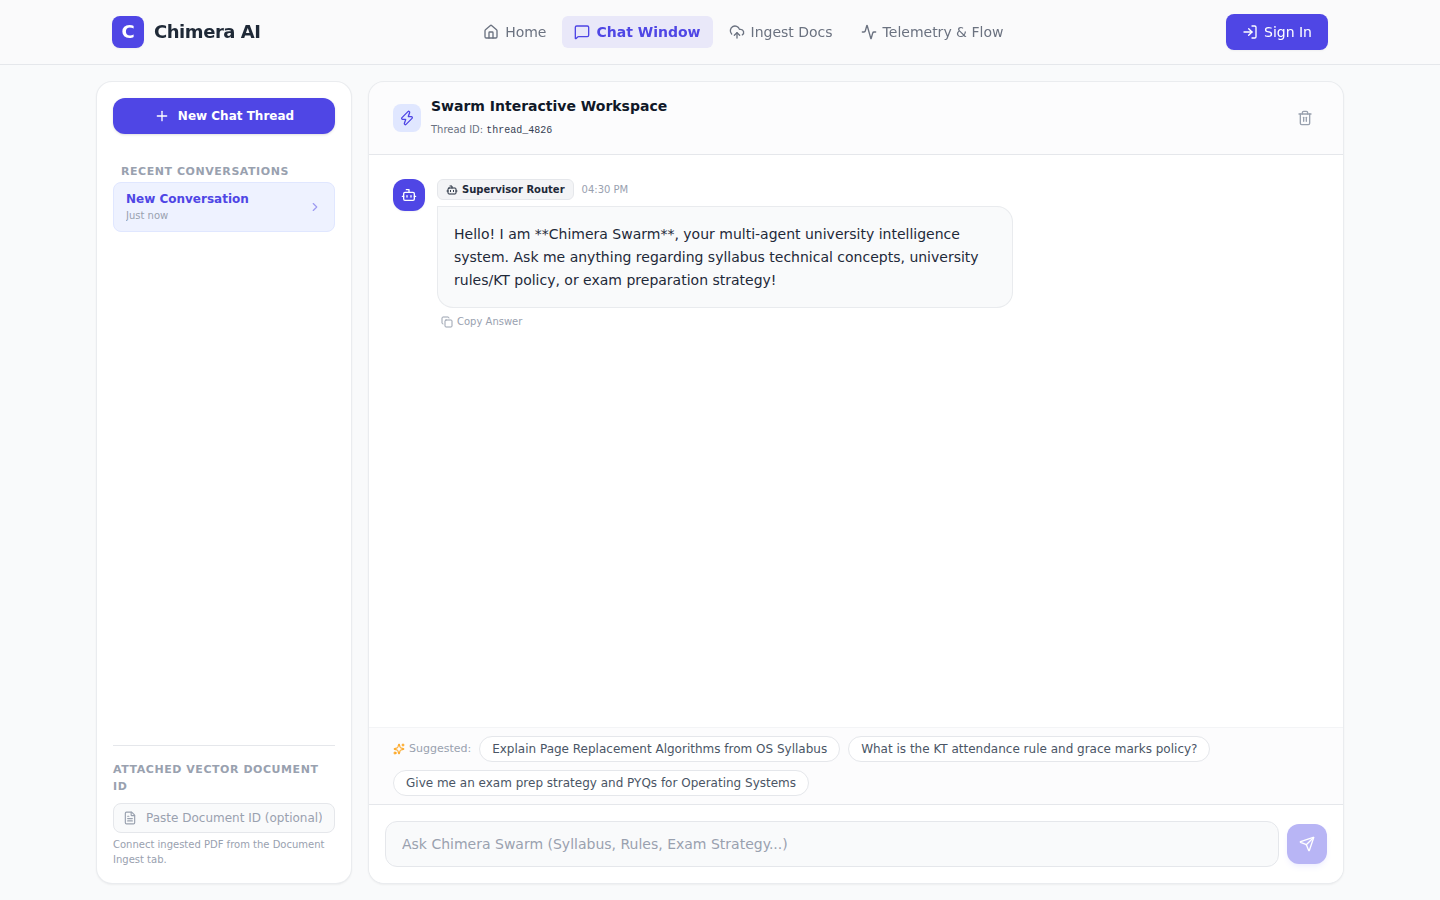
\includegraphics[width=0.82\textwidth]{images/chat.png}
\caption{Interactive Chat Page showing Real-Time Streaming and Agent Badges}
\label{fig:chat}
\end{figure}

\subsection{3. Vector Document Ingestion Portal}
The Ingest Page (\texttt{/ingest}) allows students and faculty to upload custom PDF syllabi and TXT question banks. The interface provides dual upload drop-zones, real-time file upload status indicators, and background vector index processing.

\begin{figure}[htbp]
\centering
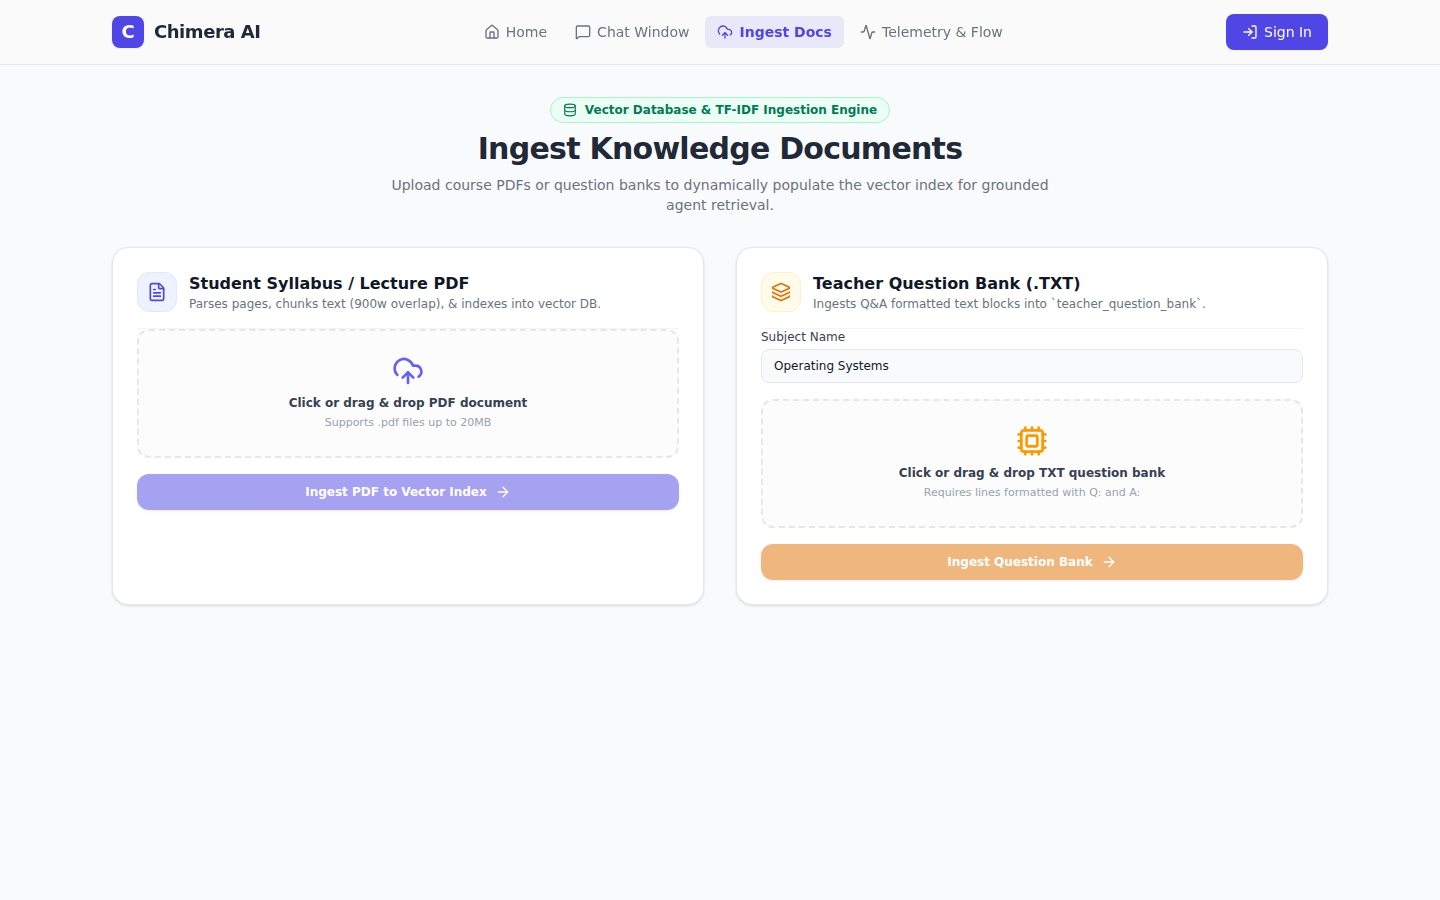
\includegraphics[width=0.82\textwidth]{images/ingest.png}
\caption{Vector Document Ingestion Portal for Syllabus and Question Bank Uploads}
\label{fig:ingest}
\end{figure}

\subsection{4. Swarm Telemetry and Event Pipeline Visualizer}
The Telemetry Page (\texttt{/telemetry}) gives users full visibility into the system's execution pipeline. It features an interactive 4-stage node visualizer (Ingress $\rightarrow$ Router $\rightarrow$ Agent Execution $\rightarrow$ Vector DB Retrieval) along with a live event log terminal displaying incoming SSE JSON payloads.

\begin{figure}[htbp]
\centering
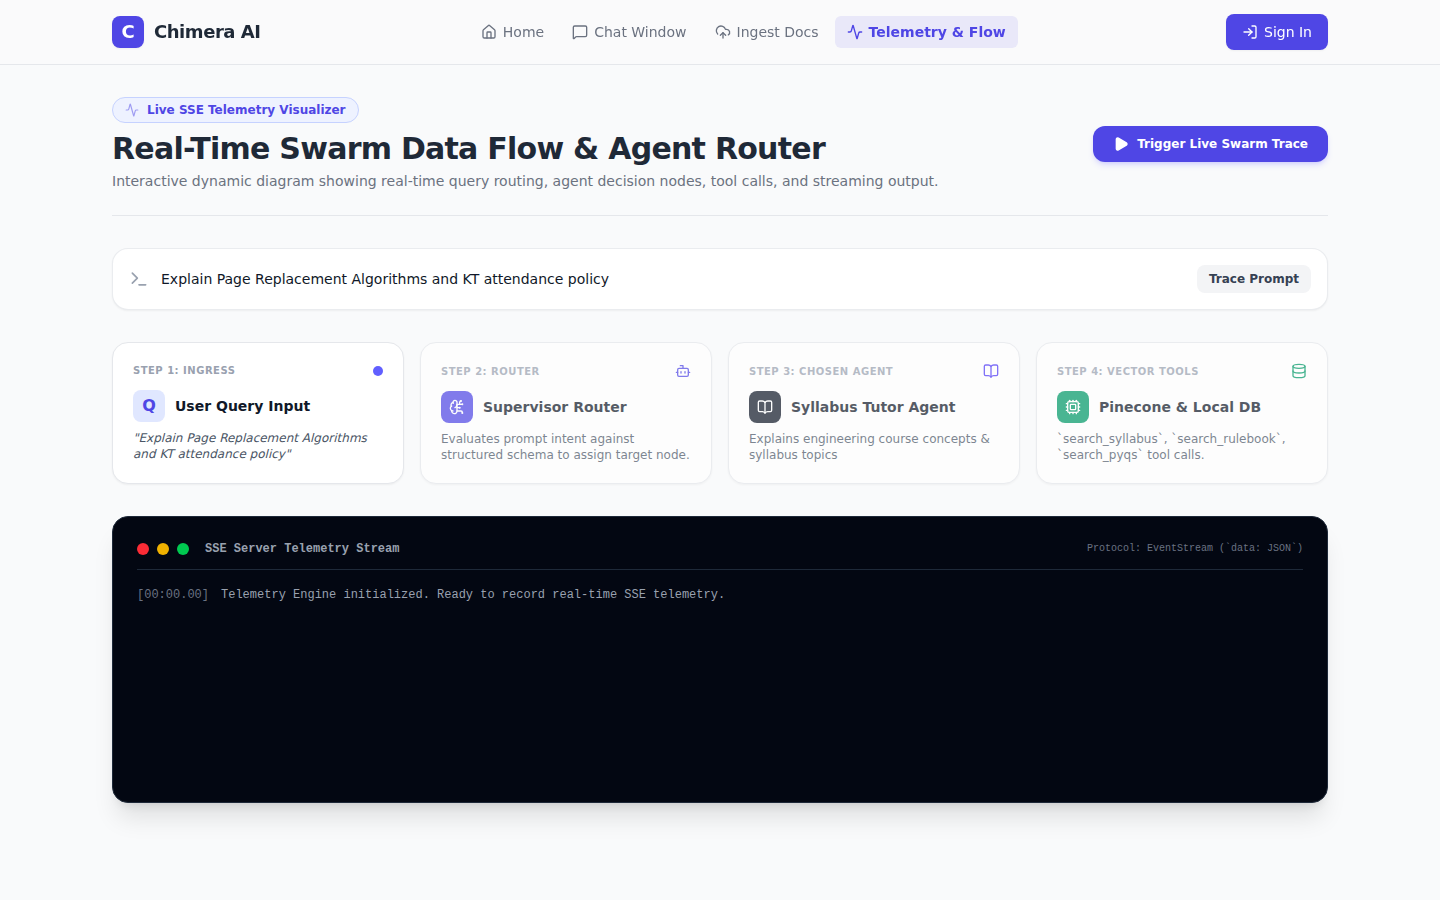
\includegraphics[width=0.82\textwidth]{images/telemetry.png}
\caption{Swarm Telemetry Visualizer showing Data Flow Nodes and Event Logs}
\label{fig:telemetry}
\end{figure}

\section{Recommendations for Optional User Diagrams}
To keep the report concise and within the 10--12 page limit, 4 core screenshots have been included above. If additional technical diagrams are required for future submissions, the following places are recommended:
\begin{enumerate}
    \item \textbf{Sequence Diagram (Chapter 3):} A diagram showing the request-response lifecycle between the React frontend, Gateway, and FastAPI backend during SSE streaming.
    \item \textbf{Database Schema Diagram (Chapter 3):} A vector database metadata diagram depicting Pinecone namespaces (\texttt{student\_documents} vs \texttt{question\_banks}).
    \item \textbf{User Flowchart (Chapter 4):} A flowchart showing user navigation from the login page to chat and ingestion portals.
\end{enumerate}
